%\newpage
\chapter{INTRODUCTION}\label{chapter_introduction}
%\pagebreak
\section{Introduction}

Handwriting Recognition is the mechanism for transforming the written text into a symbolic representation. Off-line handwriting recognition is the task of determining what characters or words are present in a digital image of handwritten text. The problem of handwriting recognition can be viewed as a classification problem where we need to identify the most suitable character the given figure matches to. It is a sub-field of \ac{ocr}, whose domain can be machine-print or handwriting but is more commonly machine-print. Handwriting Recognition plays an essential role in many human computer interaction applications including cheque verification, mail sorting, office automation, handwritten form verification, etc.

\subsection{Motivation}
Handwriting recognition is a special problem in the domain of pattern recognition and machine intelligence. The field of handwriting recognition can be split into two different categories: on-line recognition and off-line recognition.  On-line mode deals with the recognition of handwriting captured by a tablet or similar touch-screen device, and uses the digitized trace of the pen to recognize the symbol. Off-line mode determines the recognition of text images. More about on-line and off-line techniques is given in section \ref{section_online_offline}.  The problem of handwriting increases when we operate it in the off-line mode. Lots of work has been done in this area in the past few years. The motivation behind developing character recognition systems is inspired by its wide range of applications including human-computer interaction, archiving documents, automatic reading of checks, number plate reading of vehicles, etc.

\ac{ann} in the area of handwriting recognition achieves more efficiency and accuracy than using other statistical recognition tools. \ac{ann} is grabbing great attention in the field of pattern recognition due to its simple structure, high accuracy, parallel computing, fault-tolerance and self learning capacity.

Nepali handwriting recognition system can also help in automatic reading of ancient Nepali manuscripts. Automatic processing benefits into availability for their contents. Besides the advantages of automated handwriting system, image degradation, unexpected markings and previously unseen writing styles provide challenges in the recognition procedure.

\subsection{On-line versus Off-line Recognition}\label{section_online_offline}

In On-line handwriting recognition, user is directly connected to the system using an electronic pen or a touch-screen and recognition is carried out in real time. All various geometrical attributes, e.g. positions, distances, angles, curvatures and local directions have been evaluated on sample points. We also have temporal information about the character being written, such as the stroke order, pen up and pen down time, sequence of points traced, etc. High accuracy can be achieved in the case of on-line handwriting recognition, since we can extract various important geometric, statistic and temporal features from character being written.

In off-line handwriting recognition, the recognition is carried out on handwritten text that is captured using a scanner or a camera. Thus, the text is treated as an image. Off-line approach is free from stroke order variations. However, both on-line and off-line methods are similar in many aspects except for the fact that off-line methods does not have any temporal information. However, using certain heuristic methods and prior knowledge (for example in the Roman script, writing is always performed from left to right), we can determine the direction of the strokes with respect to time.

In on-line approach, the character is normally represented as a sequence of feature vectors which are extracted along the pen tip trajectories and thus exhibits some dynamic characteristics. In contrast, in off-line approach, the character is modelled by the feature vector describing the holistic shape directly.

\subsection{Nepali Natural Handwriting}
Nepali language belongs to Devanagari script which is invented by Brahmins around 11th century AD. Devanagari script is also adapted in many other languages like Hindi, Marathi, Bangali and many more. In Nepali language, there are 33 pure consonants (vyanjan) and also half forms, 13 vowels (swar), 16 modifiers and 10 numerals \cite{Santosh2007}. In addition, consonants occur together in clusters, often called conjunct consonants. Altogether, there are more than 500 different characters. According to the Nepal census, conducted by His Majesty's Government of Nepal in 2001 AD, More than 17 million speakers worldwide, including 11 million within Nepal speak Nepali language.

Nepali is written from left to right along a horizontal line. Characters are joined by horizontal bars that create an imaginary line by which Nepalese texts are suspended, often called 'shirorekha’. The single or double vertical line at the end of writing represents a completeness of one sentence which is called 'purnabiram'. A few samples of nepali handwritten characters are shown in Figure \ref{figure_sample_ka_kha}, Figure \ref{figure_sample_a_aa} and Figure \ref{figure_sample_one_two}.
\begin{figure}[hbtp]
\centering
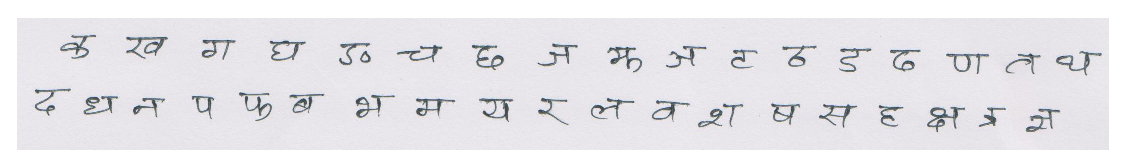
\includegraphics[width=\linewidth]{figures/datasets/nhcr/ka_kha.eps}
\caption{Sample of Nepali Handwritten Consonants.}
\label{figure_sample_ka_kha}
\end{figure}
\begin{figure}[hbtp]
\centering
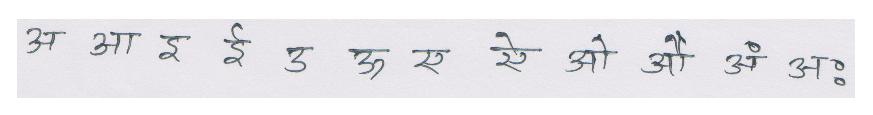
\includegraphics[width=\linewidth]{figures/datasets/nhcr/a_aa.eps}
\caption{Sample of Nepali Handwritten Vowels.}
\label{figure_sample_a_aa}
\end{figure}

\begin{figure}[hbtp]
\centering

\includegraphics[width=\linewidth]{figures/datasets/nhcr/one_two.eps}
\caption{Sample of Nepali Handwritten Numerals.}
\label{figure_sample_one_two}
\end{figure}

\subsection{Application of Off-line Nepali Handwriting Recognition System}

The main industrial applications for the recognition of off-line handwritten text are currently found in the area of address reading and bank cheque processing, where recognition is based on digitized images of physical envelopes or bank cheques.

Applications for off-line recognition of unconstrained handwritten text may be found in the future to the automatic recognition of personal notes and communications. Recognition rate of current systems in the off-line, writer independent case are still far from being perfect.

The automatic transcription of large handwritten archives seems a more realistic scenario today. Such applications could support automatic indexing for information retrieval systems used in digital libraries which do not require perfect recognition rates.

Making handwritten texts available for searching and browsing is of tremendous value.
To digitalize the historic documents written in ancient time, off-line Nepali handwriting recognition plays a good role. Indexing of handwritten documents for searching and sorting is another application area of off-line Nepali Handwriting recognition.

\subsection{Human performance in recognizing Handwritten Texts}
Most people can read handwritings with word recognition rates of $100\%$ if they are familiar with that particular language. Human performance will be often poor, if a letter by letter recognition is required. The knowledge of the possible vocabulary and frequently used word sequences (word n-grams) can help to improve the word recognition rate. However, optimal transcriptions of handwritten texts can be expected if the reader is familiar with both the language and the topic of the text, i.e. if the text is actually understood.

It can generally be observed that the amount of task specific knowledge has a significant impact on the resulting system performance.

\subsection{Artificial Neural Networks}
Artificial neural network is non-linear, parallel, distributed, highly connected network having capability of adaptivity, self-organization, fault tolerance, evidential response and \ac{vlsi} implementation, which closely resembles with physical nervous system. Physical nervous system is highly parallel, distributed information processing system having high degree of connectivity with capability of self learning. Human nervous system contains about 10 billion neurons with 60 trillions of interconnections. These connections are modified based on experience. Typical physical neuron is given in figure \ref{figure_physical_neuron} and artificial neuron is given in figure \ref{figure_artificial_neuron}.

\begin{figure}[ht]
\begin{minipage}[b]{0.5\linewidth}
\centering
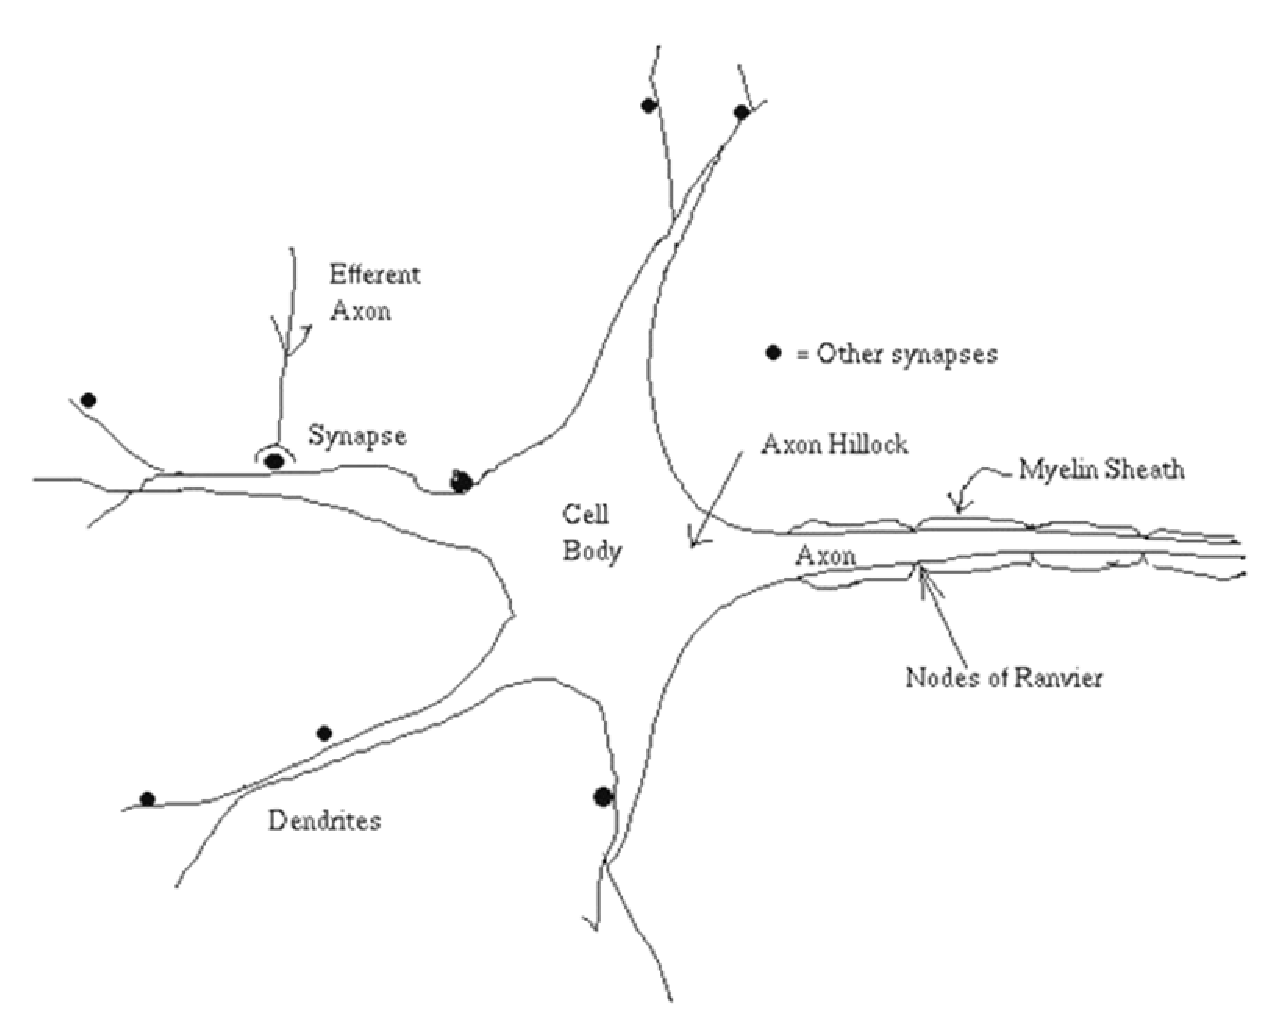
\includegraphics[scale=0.40]{figures/ann/physical_neuron.eps}
\caption{A Physical Neuron.}
\label{figure_physical_neuron}
\end{minipage}
\hspace{0.5cm}
\begin{minipage}[b]{0.5\linewidth}
\centering
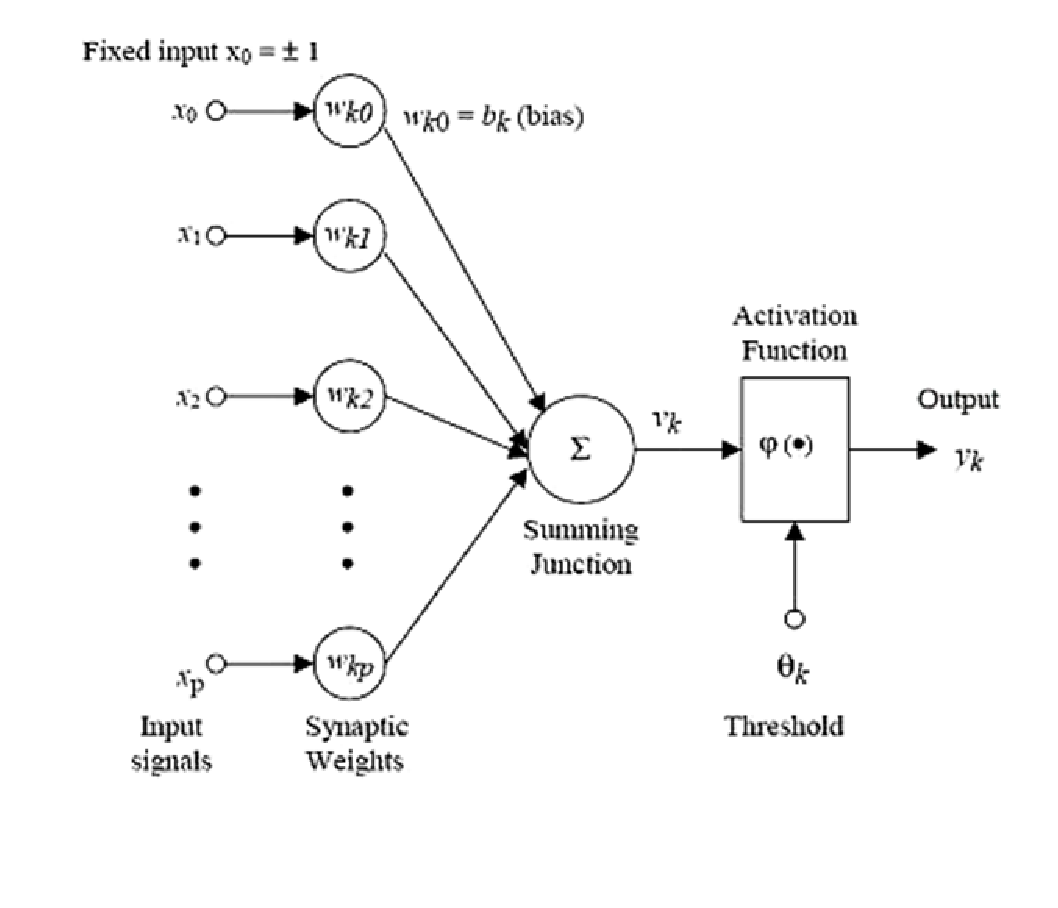
\includegraphics[scale=0.40]{figures/ann/artificial_neuron.eps}
\caption{An Artificial Neuron.}
\label{figure_artificial_neuron}
\end{minipage}
\end{figure}

Artificial neural networks are composed of interconnecting artificial neurons (programming constructs that mimic the properties of biological neurons). Artificial neural networks may either be used to gain an understanding of biological neural networks, or for solving artificial intelligence problems without necessarily creating a model of a real biological system. The real, biological nervous system is highly complex. Artificial neural network algorithms attempt to abstract this complexity and focus on what may hypothetically matter most from an information processing point of view. Good performance (e.g. as measured by good predictive ability, low generalization error), or performance mimicking animal or human error patterns, can then be used as one source of evidence towards supporting the hypothesis that the abstraction really captured something important from the point of view of information processing in the brain. Another incentive for these abstractions, is to reduce the amount of computation required to simulate artificial neural networks, so as to allow one to experiment with larger networks and train them on larger data sets.

\subsubsection{History of Artificial Neural Networks}
The modern view of neural network began in the 1940s with the work of Warren McCulloch and Walter Pitts, who showed that networks of artificial neurons could, in principle, compute any arithmetic or logical function.

McCulloch and Pitts were followed by Donald Hebb, who proposed that classical conditioning (as described by Pavlov in the experiment of food presenting to the dog) is present because of the properties of individual neurons. Hebb proposed a mechanism for learning artificial neurons in the way of biological neurons.

The first practical application of the artificial neural networks came in the late 1950s, with the invention of the perceptron network and associative learning rule by Frank Rosenblatt \cite{Haykin1999} .

Around 1956, Bernard Widrow and Ted Hoff introduced a new learning algorithm and used to train adaptive linear neural networks, which is similar in structure and capability to Rosanblatt’s perceptron \cite{Hagan1996} . Another system besides perceptron was the \ac{adaline} which was developed in 1960 by Widrow and Hoff (of Stanford University).

Rosenblatt’s and Widrow’s network both suffer from limitation of applicability of networks only to linearly seperable classes of problems. Limitations of these networks were publicized in the book by Marvin Minsky and Seymour Papert with the fact that there were no powerful digital computers to do experiments. So, for a decade, neural network research was largely suspended.

Development of neural network dramatically increased from 1980, as there were powerful personal computers to do experiments and the development of multilayer backpropagation perceptron network. The most influenced publication of the backpropagation algorithm was by Devid Rumelhart and James Mclelland. This algorithm was the answer to the criticisms Minsky and Papert had made in the 1960s.

Significant progress has been made in the field of neural networks-enough to attract a great deal of attention and fund further research. Advancement beyond current commercial applications appears to be possible, and research is advancing the field on many fronts. Neurally based chips are emerging and applications to complex problems developing. Clearly, today is a period of transition for neural network technology.
\subsubsection{Real Life Applications of Artificial Neural Networks}
Some real life applications of Artificial Neural Network are given below.

\begin{itemize}
\itemsep0em
\item Signal processing (e.g. adaptive echo cancelling).
\item Control (e.g. manufacturing plants for controlling automated machines).
\item Robotics (e.g. vision recognition).
\item Pattern recognition (e.g. recognizing handwritten characters).
\item Medicine (e.g. storing medical records based on case information).
\item Speech production (e.g.reading text aloud).
\item Speech recognition.
\item Vision (e.g. face recognition).
\item Business (e.g. rules for mortgage decisions).
\item Financial Applications (e.g. stock market prediction).
\item Data Compression (e.g. images).
\item Game Playing (e.g. chess).
\end{itemize}
%Application areas of ANNs include system identification and control (vehicle control, process control), game-playing and decision making (backgammon, chess, racing), pattern recognition (radar systems, face identification, object recognition), sequence recognition (gesture, speech, handwritten text recognition), medical diagnosis, financial applications, data mining (or knowledge discovery in databases, "KDD"), visualization and e-mail spam filtering.

\section{Challenges}
Unconstrained off-line handwriting recognition has significantly different writing styles and shapes. Shapes of the same character glyph vary across writers and even for the same writer. General handwritten text document can have large variations on writings. Same Character, word or sentence  can have different writing styles, alignment styles, skewness and slantness for the same document. It makes handwriting recognition more complicated.

Off-line handwritten text recognition can be seen as the most general case of handwriting recognition. Complexity of handwriting recognition system vary according to its problem domain ( e.g., Number plate recognition, Cheque verification, Digit recognition, etc...). Writer Recognition is much more difficult than  Writer Independent Handwriting Recognition. So, unconstrained off-line handwriting recognition is a very challenging problem in the domain of pattern recognition and artificial intelligent.

%Different, or even the same writer can write differently at different times, depending on the pen or pencil, the width of the line, the slight rotation of the paper, the type of paper and the mood and stress level of the person

\section{Problem Definition}
The high-level task of off-line handwriting recognition is to classify the ordered sequence of images of off-line characters. In this research work, problem of Nepali handwritten character recognition is addressed. This corresponds to the ability of human beings to recognize such characters, which they are able to do with little or no difficulty. The recognition task is carried out with Artificial Neural Network. Many geometric and statistical features are extracted from images so that the performance and accuracy of recognition system is achieved in the range of human ability of recognition. The system performs character recognition by quantification of the character into a mathematical vector entity using the geometrical and statistical properties of the character image.  The sub problems in the domain of off-line handwriting recognition such as, noise removal, image binarization, object skeletonization, size normalization, etc. have great impact on recognition procedure. These sub-problems are also addressed with the most suitable solutions in the literature for this type of research work.

\section{Objectives}
The objective of this research is to investigate various feature extraction techniques and to compare Neural Network based pattern recognition techniques namely Multilayer Feed-forward Network and Radial Basis Function Network. Comparative Performance matrices are analysed. The sub-problem field of off-line handwriting recognition is also addressed. Main objectives are given below.
\begin{itemize}
\item  To compare performance and efficiency of \ac{mlp} and \ac{rbf} Neural Networks on Off-line Nepali Handwriting Recognition Problem.
\item To investigate Geometric and Statistical feature extraction techniques for off-line Nepali handwritten text.
\item To investigate preprocessing techniques (segmentation, skeletonization, normalization, etc.) for handwritten documents.
\item To create benchmark databases for Nepali handwritten characters.
\end{itemize}

\section{Contribution of this Thesis}
The main contribution of this thesis to the field of Off-line Nepali Handwriting Recognition can be seen in its extensive experimental work. A more detailed list of the various contributions is provided below,

\begin{itemize}
\itemsep0em
\item Use of ANN to analysis the off-line handwriting recognition problem.
\item Investigation of feature extraction techniques for off-line handwritten documents.
\item Creation of Nepali Handwritten character database for the experimentation with the recognition system.
\end{itemize}

\section{Outline of the Thesis}
The remaining part of the document is organized as follows,\par

\textbf{Chapter \ref{chapter_literature_review}} describes the state of the art of the handwriting recognition. It includes the methods and techniques used in the area of handwriting recognition till now.\par

\textbf{Chapter \ref{chapter_system_overview}} describes the Off-line Handwriting Recognition System architecture. The Top level system overview along with sub-system engines are given with data flow directions.\par

\textbf{Chapter \ref{chapter_research_methodology}} describes research methodologies used in the research. All the preprocessing, feature extraction and recognition algorithms are described in this part of the document.\par

\textbf{Chapter \ref{chapter_implementation}} describes the implementation of the system. It includes the techniques used for the realizations of the algorithms given in chapter \ref{chapter_research_methodology}.

\textbf{Chapter \ref{chapter_nepali_handwritten_database}} describes the corpus used in the evaluation of the purposed system. Off-line handwriting recognition system is experimented with three self created Nepali handwritten character datasets for consonants, vowels and numerals respectively.

\textbf{Chapter \ref{chapter_experimentation_and_results}} describes the experimentation results of the recognition systems. Performance and efficiency of the proposed systems evaluated in Nepali handwritten character datasets are given in this section.

\textbf{Chapter \ref{chapter_conclusion}} contains the summary and future scope of the research work.
